\subsection{Проектирование и разработка клиентской части программного средства}
\label{sec:design:client}

Задачи клиентской части приложения включают отображение пользовательского интерфейса и обработку действий пользователя. Типичными этапами его проектирования являются следующие~\cite[с.~78]{application_architecture_guide}:

\begin{itemize}
	\item Идентификация типа клиентской части приложения, которое удовлетворяет установленным требованиям. Осуществление данного этапа осуществлено в подразделе~\ref{sec:design:architecture}.
	\item Выбор технологии пользовательского интерфейса. Осуществляется на основе анализа требуемой для реализации функциональности.
	\item Проектирование UI. Хорошей практикой является реализация модульности, а также принципа разделения ответственности компонентов.
	\item Определение стратегии и протоколов обмена информации между уровнями. Поскольку рассматриваемый уровень является самым верхним, а его протоколы связи с серверной частью приложения были рассмотрены в пункте~\ref{sec:design:server:protocols}, то данный вопрос считается решенным и рассматриваться не будет.
\end{itemize}

Ранее был проведен анализ и осуществлен выбор целевой платформы для реализации клиентской части приложения, был выбран основной язык программирования. Однако, существует огромное число специализированных технологий и фреймворков по созданию пользовательских интерфейсов. Представляется целесообразным провести уточнение средств разработки.

\subsubsection{} Уточнение выбора технологий программирования
\label{sec:design:client:technologies}

Язык программирования \typescript является надмножеством языка \js. Основной его особенностью является наличие проверок типов во время компиляции. Обычный \js код может быть скомпилирован \typescript компилятором (на выходе получится тот же самый код), однако по умолчанию данная возможность выключена, компилятор будет производить ошибку. Тем не менее, у разработчиков программного обеспечения есть возможность использования неимоверно большого числа \js библиотек и фреймворков, которая заключается в создании и использовании специальных файлов (их принято создавать с расширением .d.ts), которые содержат определения типов (type definitions) и создаются для каждой предназначенной к использованию библиотеки. Определенную проблему может представлять создание таких файлов: они бывают довольно громоздкими и их создание требует некоторых временных затрат. Тем не менее, существует проект по созданию таких файлов обычными разработчиками~\cite{github_definitelytyped}. В репозитории данного проекта находятся уже созданные .d.ts файлы для огромного числа существующих библиотек, что означает, что \typescript разработчики глубоко интегрированы в экосистему \js разработки.

Одной из широко используемых в настоящее время библиотек по созданию интерактивных интерфейсов веб-приложения является библиотека \react. Выбор в ее пользу был осуществлен вследствие наличия опыта по ее использованию у членов команды. Особенностями данной библиотеки являются следующие~\cite{habr_react_introduction}:

\begin{itemize}
	\item Кроссплатформенность. Переиспользование существующего кода\linebreakвозможно даже на других платформах благодаря проекту React Native.
	\item Декларативность: использование элементов (стандартных для \react \linebreak объектов, которые представляют собой HTML-теги) и компонентов (объекты, создаваемые разработчиком).
	\item JSX: техника создания и использования компонентов с помощью\linebreak HTML-подобного синтаксиса, который применяется прямо в \js коде.
	\item Виртуальный DOM: дерево \react элементов, которое отрисовывается в браузере, причем изменения в нём не требуют полной перерисовки всего интерфейса. Позволяет значительно улучшить быстродействие при использовании библиотеки.
\end{itemize}

Строго говоря, использование JSX является опциональным и может как не использоваться при разработке с \react, так и использоваться при разработке с помощью других библиотек. Однако, он значительно упрощает исходный код компонентов. Например, следующий \js код 
\begin{flushleft}
\qquad\qquad\qquad return <div>Hello\{this.props.children\}</div>;
\end{flushleft}
после компиляции будет преобразован в следующий
\begin{flushleft}
\qquad\qquad\qquad return React.createElement(\\
\qquad\qquad\qquad\qquad ``div'',\\
\qquad\qquad\qquad\qquad null,\\
\qquad\qquad\qquad\qquad ``Hello '',\\
\qquad\qquad\qquad\qquad this.props.children\\
\qquad\qquad\qquad );
\end{flushleft}

Лаконичность использования JSX очевидна. Некоторым кажется сомнительным данный подход, в котором смешивается исполняемый код и код разметки. Однако, данное смешение формирует исходный код представления. Кроме того, в других фреймворках используются специальные конструкции по реализации, например, циклов, условий, в то время как при использовании JSX нужды в новых конструкциях нет, ведь используются стандартные операторы языка \js (в текущем проекте -- \typescript).

Одна из классификаций компонентов \react предполагает их разделение на pure (простые) и stateful (имеющие внутреннее состояние)~\cite{react}. Простые компоненты, реализованные в виде классов, унаследованных от Re\-act.Com\-po\-nent, переопределяют метод render(), который принимает некоторый набор исходных данных и возвращает элемент, предназначенный для отображения. Компоненты другого класса имеют внутри себя некоторые данные, образующие их состояние. Чтобы \react узнал, что данные изменились, и осуществил перерисовку измененных компонентов, требуется использовать специальный метод this.setState(...). 

Для упрощения управления состоянием компонентов могут применяться различные техники. Одной из них является использование специальной библиотеки \mobx. Его идея заключается в недопущении неконсистентного состояния приложения, что достигается отслеживанием данной библиотекой всего дерева используемых объектов и обновлении интерфейса при любом их изменении. Рекомендуемый и наиболее удобный способ использования \mobx заключается в использовании специальных декораторов, с помощью которых помечаются классы, методы и поля классов. Не смотря на их официальный экспериментальный статус, они поддерживаются компилятором \typescript. В терминологии \mobx существуют следующие объекты программы:

\begin{itemize}
	\item \react компонент, который автоматически перерисовывается при изменении состояния. Помечается декоратором @observer.
	\item Объекты в классах, находящиеся под наблюдением библиотеки. Обозначаются с помощью декоратора @observable.
	\item Вычисляемые методы, возвращающие некоторое значение на основании состояния объекта или других вычисляемых методов. Подвергаются оптимизации со стороны \mobx. Обозначаются декоратором @computed.
	\item Методы, изменяющие состояние объектов. Обычно это некоторые операции ввода-вывода, а также передачи данных. Помечаются с помощью @ac\-ti\-on.
	\item Методы, которые должны автоматически запускаться при любых изменениях содержащихся в них данных. Типичный пример их использования: логгирующие операции. Обозначаются с помощью @autorun.
\end{itemize}

Однако, \mobx представляет собой только библиотеку. Ограничения на архитектуру приложения не накладываются, однако сохраняется\linebreak необходимость ее реализации программистом. Одним из вариантов является разбиение всех компонентов на контейнерные и презентационные~\cite{presentational_and_container_components}. Особенности создания презентационных компонентов следующие:

\begin{itemize}
	\item Их задача заключается в определении, как должны \emph{выглядеть} элементы.
	\item Не зависят от других частей приложения.
	\item Получают данные исключительно в качестве входных параметров.
	\item Не изменяют данные.
	\item Редко имеют собственное состояние (в таком случае это состояние UI, а не собственно данные).
	\item Обычно содержат JSX разметку и имеют относящиеся к ним стили.
\end{itemize}

В это же время особенности контейнерных компонентов заключаются в следующем:

\begin{itemize}
	\item Их задача заключается в определении, как элемент должны \emph{работать}.
	\item Предоставляют данные и методы их обработки другим компонентам.
	\item Как правило имеют некоторые данные в виде состояния.
	\item Обычно не содержат JSX разметки и никогда не имеют стилей.
\end{itemize}

Использование данного подхода имеет следующие преимущества:

\begin{itemize}
	\item Достигается выполнение принципа разделения ответственности.
	\item Появляется возможность легкого переиспользования компонентов с\linebreak различными источниками данных.
	\item Одни и те же презентационные компоненты могут использоваться повсеместно в приложении.
	\item Презентационные компоненты формируют <<палитру>>. Их внешний\linebreak вид может изменяться без влияния на логику приложения.
\end{itemize}

Еще один важный момент относительно проектирования UI, помимо содержания и интерактивных пользовательских взаимодействий, касается стилизации внешнего вида компонентов. Существует несколько подходов по ее исполнению~\cite{styling_react}: использование внутренних (inline) и внешних стилей.

Первый подход имеет множество недостатков:

\begin{itemize}
	\item невозможно использование медиа-запросы, чтобы, например, реагировать на изменения ширины экрана или отличать мобильное устройство от настольного компьютера;
	\item невозможно использование псевдоклассов и псевдоэлементов, например: :hover, :active, :before, :after;
	\item значительное увеличение размера разметки и снижение производительности;
	\item невозможно переопределение стилей по более сложным селекторам.
\end{itemize}

Тем не менее, Facebook, как компания разработчик \react, несмотря на описанные недостатки, выступает за использование inline стилей. Причиной этому является стремление обеспечить единообразие с React Native, поскольку там возможность стилизации обеспечивается только данным подходом.

Второй подход -- использование внешних стилей -- является более традиционным для веб-разработки. Его эволюционное развитие включает несколько этапов:

\begin{itemize}
	\item Создание одного файла .css со стилями, который подключается один раз глобально в главный html файл. В React компонентах используется тег className со значениями имен классов из этого файла.
	\item Разбиение единого файла стилей на множество файлов в соответствии с реализованными компонентами. В файлы компонентов подключаются лишь те стили, которые там необходимы. Преимущества данного подхода заключаются в простоте поиска файла, в который необходимо внести изменения, и в простоте удаления компонентов и соответствующих им файлов стилей.
	\item Использование различных препроцессоров стилей, таких как\linebreak SASS/SCSS, LESS и прочих. 
\end{itemize}

Использование SASS по сравнению с обычным CSS предоставляет следующие преимущества~\cite{sass_guide}:

\begin{itemize}
	\item переменные, в которых можно хранить значения цветов, шрифтов, а также любые другие значения;
	\item вложенность, что приводит к большей наглядности файлов стилевых таблиц за счет соответствия иерархии HTML кода;
	\item фрагментирование, то есть обеспечение модульности;
	\item импортирование других файлов стилей, которое, в отличие от CSS, вместо создания новых HTTP запросов подставляет указанный файл в тот, где он вызывается, таким образом на выходе получается единственный файл стилей;
	\item примеси (mixins), которые представляют собой группы деклараций, используемые по нескольку раз;
	\item наследование, позволяющее привносить наборы свойств от одного селектора к другому;
	\item использование математических операторов.
\end{itemize}

Таким образом, на основании проведенного уточнения технологий для использования выбираем следующие: \react в связке с \mobx и SCSS, кроме того, для разметки в коде повсеместно будет использоваться JSX.

% \sub subsection{}
% \label{sec:design:client:ui}
% 
% Пользовательский интерфейс часто проектируется на этапе разработки архитектуры. Архитектура должна описывать главные элементы формата web-страниц, GUI, интерфейс командной строки и т. д. Удобство GUI может в итоге определить популярность или провал программы. Архитектура должна быть модульной, чтобы GUI можно было изменить, не затронув бизнес-правил и модулей программы, отвечающих за вывод данных \cite[с.~44]{code_complete}. 

\subsubsection{} Настройка инструмента сборки проекта
\label{sec:design:client:webpack}

Рассмотренные технологии достаточно разнородны, применяются для решения различных задач. Тем не менее их согласованное взаимодействие обеспечивает правильность работы всего приложения. Для его реализации могут использоваться различные средства, однако стандартом индустрии является \webpack. 

\webpack представляет собой инструмент для сборки веб-приложений. Главная его задача состоит в объединении большого числа файлов исходного кода в один, что значительно улучшает производительность за счет необходимости клиента загружать единственный файл. Однако его возможности далеко не ограничиваются одной лишь сборкой.

Его настройка производится с помощью специального конфигурационного файла webpack.config.js. Содержание файла, используемого в данном дипломном проекте, приведено в приложении \configfilesappendix. В таблице~\ref{table:design:client:webpack:options} приведено описание используемых параметров.

\begin{table}[!ht]
\caption{Параметры инструмента сборки \webpack, используемые в проекте}
\label{table:design:client:webpack:options}
\centering
	\begin{tabular}{{ 
	|>{\centering}m{0.3\textwidth} | 
	 >{\raggedright\arraybackslash}m{0.64\textwidth}|}}

  	\hline
  	Название параметра & {\begin{center} Описание \end{center}} \\

  	\hline
  	entry & Указывает главный файл исходного кода (так называемая точка входа в приложение).\\

  	\hline
  	output & Выходной файл, производимый в результате сборки проекта. Именно его необходимо подключать в главном HTML файле.\\

  	\hline
  	devtool & Способ создания карт кода (source maps). Применяется при отладке приложения для ускорения нахождения проблемных участков кода. \\

  	\hline
  	resolve.extensions & Позволяет в исходном коде в конструкциях import не указывать расширения файлов. \\

  	\hline
  	resolve.modules & Указывает директории, в которых должен осуществляться поиск импортируемых файлов. \\

  	\hline
  	module.rules & Указывает набор и порядок запуска загрузчиков (loaders). \\

  	\hline
  	externals & Позволяет не включать некоторые библиотеки в окончательную сборку. Предполагается, что данные библиотеки будут доступны во время исполнения. \\

  	\hline
  	devServer & Настройки отладочного сервера. \\

	\hline
	\end{tabular}
\end{table}

Как было упомянуто ранее, основная задача \webpack состоит в сборке всех файлов исходного кода проекта в один. Данная процедура осуществляется с помощью загрузчиков (loaders). Большая их часть разрабатывается открытым сообществом разработчиков. Их использование обязательно в проектах, в которых используются файлы исходного кода, не являющихся обычными \js файлами. 

Основной язык программирования данного проекта -- \typescript. В связи с этим необходимо подключить специальный загрузчик (ts-loader), который бы компилировал файлы с исходным кодом. Однако для совместимости перед ним подключен другой загрузчик source-map-loader, который загружает карты кода и передает их указанному инструменту по их обработке (параметр devtool таблицы~\ref{table:design:client:webpack:options}). Затем в очереди обработки загрузчики, ответственные за подключение всех файлов стилей (sass/scss, css). В самую последнюю очередь с помощью file-loader загружаются вспомогательные файлы различных расширений, которые необходимы для работы специальных шрифтов, а также загрузки статических файлов, таких как картинки.

Для облегчения разработки и отладки в параметрах специфицируется средство для создания карт кода (его назначение состоит в сопоставлении файлов исходного кода выходному файлу, так что становится проще находить и отлаживать конкретные строки кода), а также специальный веб-сервер. Данный сервер (webpack-dev-server), которые позволяет производить разработку и сразу же наблюдать получаемый результат. Это достигается за счет отслеживания изменяемых файлов, их перекомпиляции на лету (Hot-Module-Replacement) и отправки сообщения браузеру на обновление страницы. Кроме того, данный сервер работает очень быстро за счет того, что он загружает всё приложение в оперативную память.

\subsubsection{} Настройка пакетного менеджера
\label{sec:design:client:npm}

В настоящее время при веб-разработке не принято реализовывать абсолютно все компоненты и всю функциональность самостоятельно. Вместо этого существует большое число сторонних библиотек, разрабатываемых миллионами разработчиков по всему миру. Стандартом индустрии является использование специальных пакетных менеджеров для управления ими. Наиболее часто используемым является npm (Node Packet Manager). 

Его настройка для конкретного проекта осуществляется с помощью конфигурационного файла package.json (содержание файла, используемого в данном дипломном проекте, приведено в приложении \configfilesappendix). В таблице~\ref{table:design:client:npm:options} приведено описание используемых параметров.

\begin{table}[!ht]
\caption{Параметры пакетного менеджера npm, используемые в проекте}
\label{table:design:client:npm:options}
\centering
	\begin{tabular}{{ 
	|>{\centering}m{0.3\textwidth} | 
	 >{\raggedright\arraybackslash}m{0.64\textwidth}|}}

  	\hline
  	Название параметра & {\begin{center} Описание \end{center}} \\

  	\hline
  	version & Версия пакета проекта. \\

  	\hline
  	name & Название пакета проекта.\\

  	\hline
  	private & Используется для предотвращения случайной публикации пакета проекта. \\

  	\hline
  	scripts & Скрипты, которые могут быть использованы для сборки и запуска проекта. \\

  	\hline
  	dependencies & Список зависимостей, необходимых для работы приложения. \\

  	\hline
  	devDependencies & Список зависимостей, необходимых для разработки и тестирования. \\

	\hline
	\end{tabular}
\end{table}

Самыми важными параметрами являются version и name: без них проект даже не будет запускаться. Параметр private запрещает публикацию кода проекта в открытые базы библиотек. 

Параметр scripts специфицирует команды, с помощью которых может быть запущена компиляция, сборка и запуск проекта. Следующая команда
\begin{flushleft}
\qquad\qquad\qquad\qquad\qquad npm start webpack
\end{flushleft}
производит сборку проекта, а затем погружается в режим слежения, который рекомпилирует исходные файлы в случае их изменения. Можно заметить, что даже инструмент сборки \webpack подключается в качестве зависимости (dev\-De\-pen\-den\-cy). 

Другой пример: следующая команда
\begin{flushleft}
\qquad\qquad\qquad\qquad\qquad npm start run
\end{flushleft}
осуществляет запуск отладочного сервера (описание его работы приведено в пункте~\ref{sec:design:client:webpack}). Для запуска данных команд прямо из среды разработки Visual Studio может использоваться специальное расширение NPM Task Runner.

\subsubsection{} Проектирование клиентской части приложения
\label{sec:design:client:ux}

Далее рассмотрим вопрос взаимодействия пользователя с клиентской частью приложения. Известно, что удобство пользования программным средством может во многом определять успешность проекта в целом~\cite[с.~44]{code_complete}.

Схема работы клиентской части программной системы представлена на рисунке~\ref{fig:design:client:ux:client_algorithm}. Среди ее особенностей можно выделить в высокой степени соответствие диаграмме прецедентов, которая была составлена и рассмотрена в пункте~\ref{sec:domain:model:use_cases}. Кроме того, данный чертеж представляет собой отображение чертежа схемы серверной части с отличием в том, что там делается акцент на взаимодействие с базой данных, а в данном чертеже -- на отображении данных и интерактивном взаимодействии с пользователем. 

\begin{sidewaysfigure}
\centering
	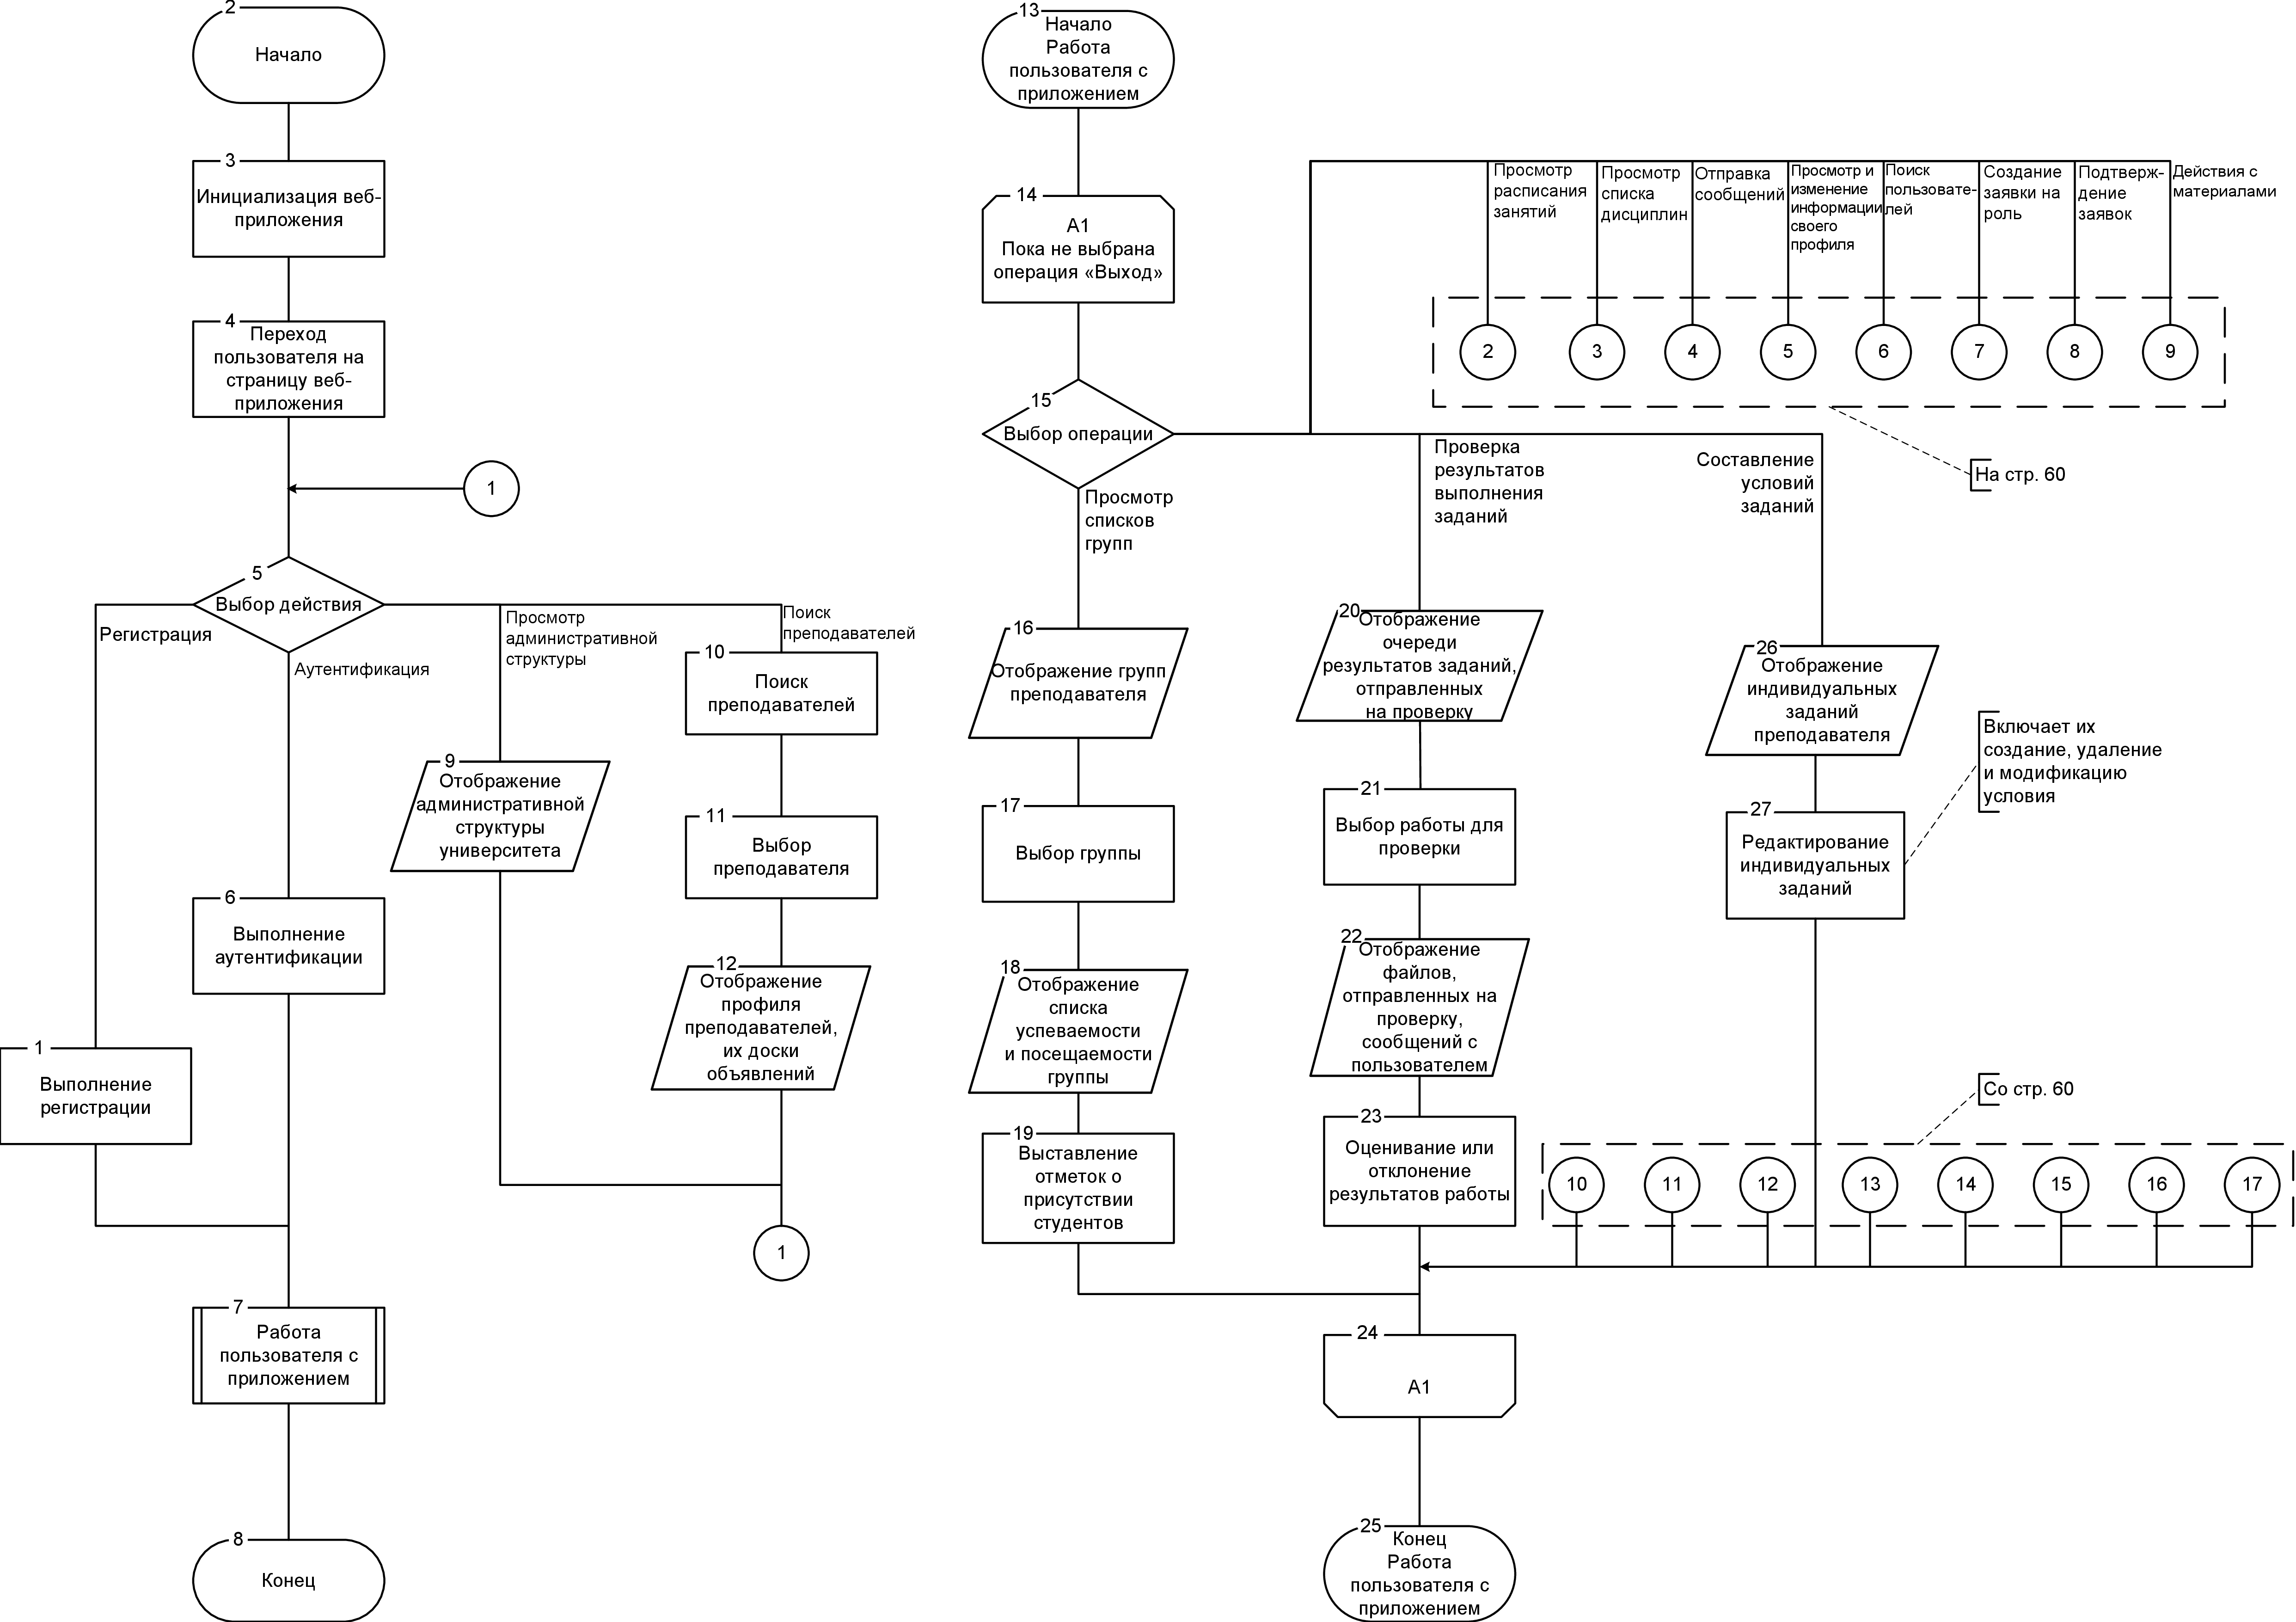
\includegraphics[scale=0.275]{client_algorithm_1.png}
	\caption{Схема программы клиентской части программного средства}
	\label{fig:design:client:ux:client_algorithm}
\end{sidewaysfigure}

\begin{sidewaysfigure}
\ContinuedFloat
\centering
	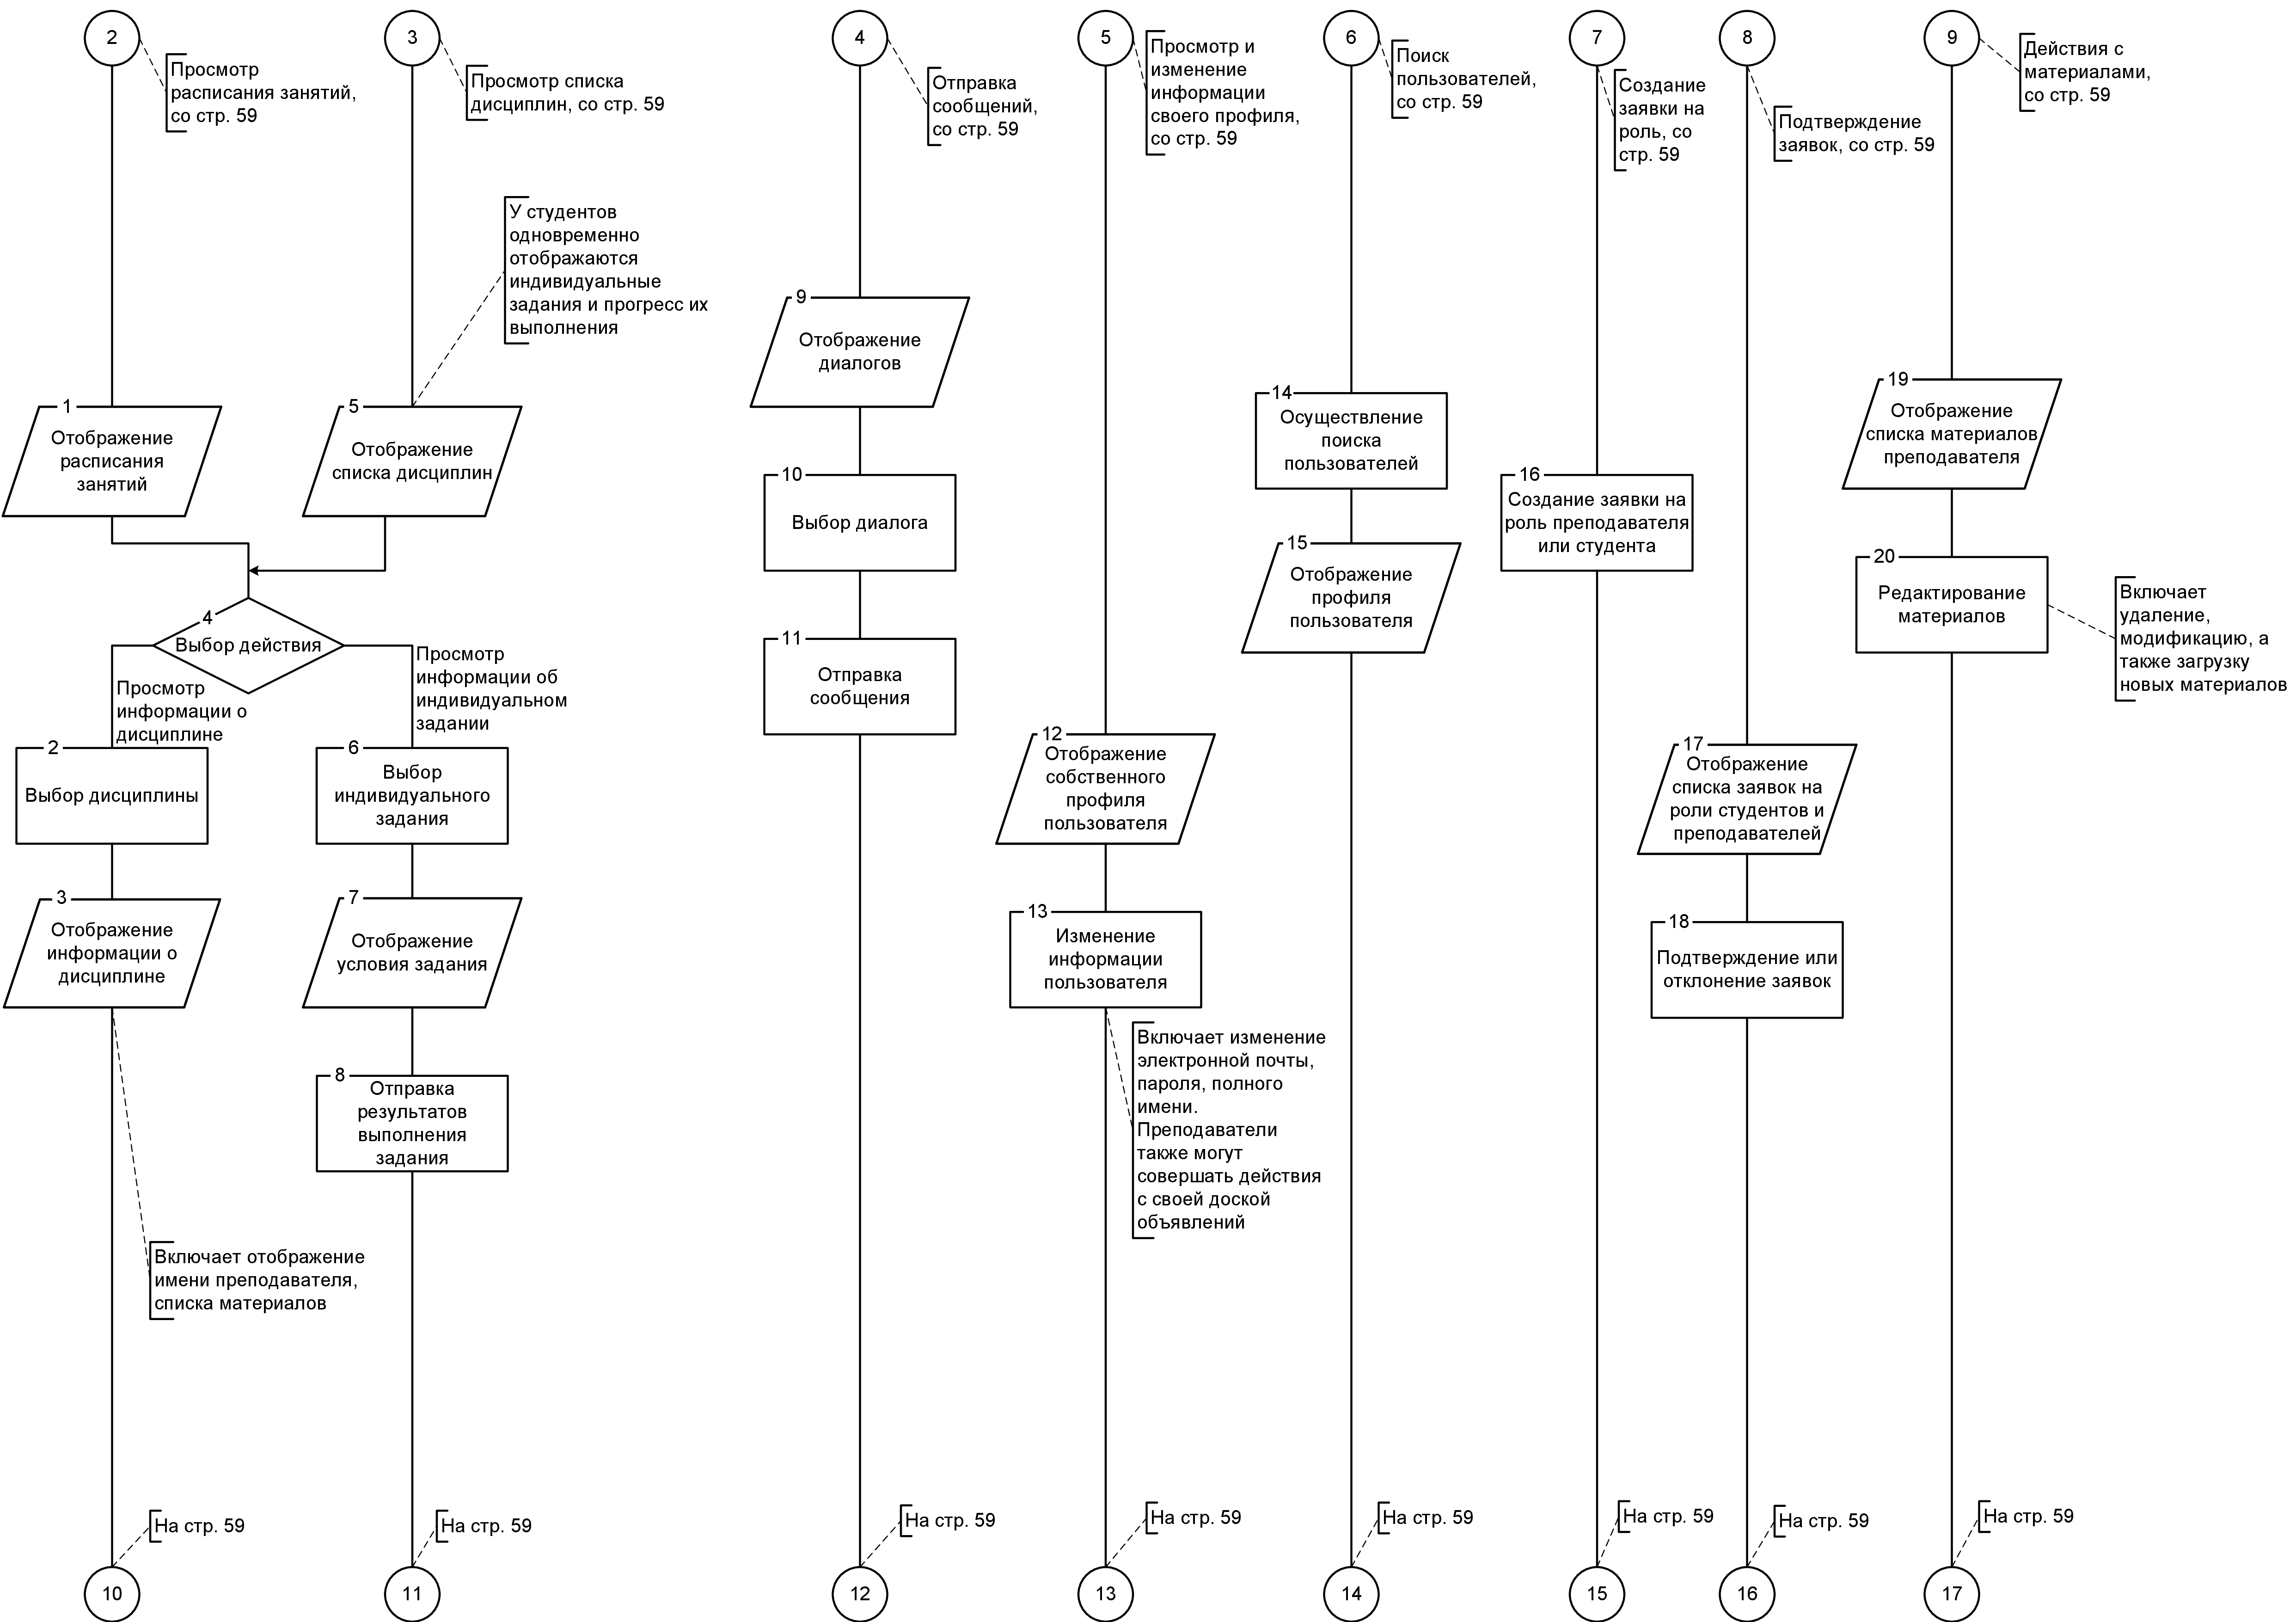
\includegraphics[scale=0.275]{client_algorithm_2.png}
	\caption{Схема программы клиентской части программного средства (окончание)}
\end{sidewaysfigure}

Таким образом, составленная схема клиентской части ПС будет использована при разработке навигации (routing) по страницам веб-приложе\-ния.

\subsubsection{} Конструирование клиентской части приложения
\label{sec:design:client:development}

Наконец, по завершению этапов проектирования и подготовки можно приступить к собственно созданию исходных кодов приложения. Ключевые фрагменты кода, описание которых приведено в данном пункте, приведены в приложении \sourcecodeappendix.

Для начала необходимо создать корневой файл index.html. Ключевая его особенность состоит в следующем теге
\begin{flushleft}
\qquad\qquad\qquad\qquad\qquad <div id=``root''></div>
\end{flushleft}

Несмотря на то, что он объявляется пустым, именно в него библиотека \react подставит всё приложение.

Кроме этого, в данном файле подключается основная зависимость приложения -- непосредственно сама библиотека \react и библиотека по управлению виртуальным деревом элементов браузера, а также пакет bun\-dle.js, в который будет собран весь созданный исходный код. Помимо библиотек, подключаются некоторые файлы стилей, необходимые для корректной работы некоторых компонентов, например, специальных шрифтов, предоставляющих возможность использования большого количества специальных иконок.

Следующий важный файл -- корневой файл исходного \typescript кода index.tsx. Единственная его цель -- вызов специального метода React\-DOM.ren\-der(), который и подставляет в указываемый тег каркас приложения.

Каркас приложения, определенный в файле App.tsx, представляет собой класс AppRouter, в котором и задаются пути маршрутизации страниц веб-приложения. В нем используется стандартный элемент Router, который при переходе пользователем по адресам приложения создаёт экземпляр класса App и передает в качестве его содержимого соответствующую страницу.

Задача компонента App -- рендеринг шапки сайта и бокового меню. В качестве дочерних для него \react подставляет такие компоненты, как Agenda (отображающий список расписания занятий), Disciplines (отображающий список дисциплин) и другие.

В качестве решения по организации пользовательского интерфейса был принят шаблон, состоящий из двух колонок. Таким образом, в левой колонке будут отображаться списки, а в правой -- детали выбранного из списка элемента. Кроме того, для повышения удобства пользования было выдвинуто требование, чтобы правая колонка не изменяла содержимого при переходах пользователем по страницам приложения. Данное требование удовлетворяется в связи с использованием библиотеки \react, поскольку она достаточно эффективно реализует механизм перерисовки только измененных областей. 

Задача дочерних компонентов класса App состоит в обращении к классам, обеспечивающим сетевое взаимодействие с сервером, получении от них данных, а затем создании <<чистых>> (pure) компонентов, которые эти данные отображают. При этом разработка производится путем движения сверху-вниз (от общих компонентов к очень маленьким частным), причем достигается высокая степень модульности: число уровней иерархии достигает не менее трех, и только самые частные компоненты отвечают за непосредственный вывод информации.

За хранение данных, а также их извлечение отвечают специальные классы, называемые <<хранилищами>> (stores). Данный подход предлагается в качестве лучших практик разработчиками библиотеки \mobx~\cite{mobx_best_practices}. Предлагаемый ими подход заключается в создании специальных классов, называемых хранилищами предметной области (domain stores), ответственных за определенные аспекты работы приложения, и разделении данных между ними. В данном дипломном проекте, такими аспектами являются хранение расписания, списка предметов, сообщений и так далее. Кроме того, предлагается создание еще одного хранилища, ответственного за хранение состояния интерфейса (UiStore), которое может хранить следующую информацию: сессионные данные, текущую тему приложения, язык (locale), разрешение экрана, состояние элементов интерфейса и так далее. Например, мы будем хранить в данном классе компоненты, ответственные за левую и правую колонку приложения.

Помимо кода компонентов, необходимо создать код их стилизации. Благодаря использованию SASS/SCSS можно достигнуть такой же степени модульности, что и при реализации компонентов. Поэтому часто классы компонентов имеют единственный им соответствующий файл стилей и импортируют лишь его.

Таким образом, разработает исходные коды клиентской части приложения. 
